\subsection{Tangent Planes}
\noindent
Although the tangent lines at a point on a surface can all be different depending on from which direction one approaches a point, all of these tangent lines lie in the same plane, defining the tangent plane.
This means that the tangent plane to $z = f(x, y)$ at $(x_0,y_0)$ has the following properties:
\begin{itemize}
	\item The z-value of the tangent plane at $(x_0, y_0)$ is the same as $f(x_0, y_0)$.
	\item The value of the first-order partial derivatives of the tangent plane at $(x_0, y_0)$ should match those of $f(x_0, y_0)$.
\end{itemize}

\noindent
The general form of a plane at $(x_0, y_0, z_0)$ is
\begin{equation*}
	P(x,y) = A(x-x_0) + B(y-y_0) + z_0.
\end{equation*}
We want $P_x = f_x$ and $P_y = f_y$.
This means that $P_x = f_x = A$ and $P_y = f_y = B$.
Rewriting,
\begin{equation*}
	P(x,y) = f_x(x-x0) + f_y(y-y_0) + z_0.
\end{equation*} 
The normal vector is $\langle \pm f_x,\pm f_y, \mp 1\rangle$.
So, the point normal form of the plane is 
\begin{equation*}
	\langle -f_x, -f_y, 1\rangle \cdot \langle x-x_0, y-y_0, z-f(x_0,y_0) \rangle = 0.
\end{equation*}

\begin{figure}[H]
	\centering
	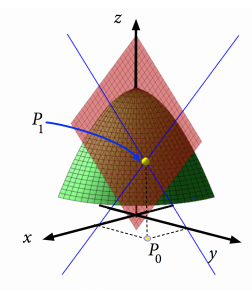
\includegraphics[width=0.5\textwidth]{./Images/differentialMultivariableCalculus/tangent_plane.png}
	\caption{Tangent plane}
\end{figure}
